% Chapter 1

\chapter{2D Plate} % Write in your own chapter title
%\label{Chapter3}
\lhead{Chapter 3. \emph{Results}} % Write in your own chapter title to set the page header

\section{Wave behaviour}
% \begin{itemize}
% \item how do I quantify a good wave - is there a correspondence between this convergence and wave shape convergence? So does this mean I can do convergence in terms of wave shapes maybe? EEEEK.
% \item do a LOT of high-p short runs to try and identify a convergence between multiple waves.
% \end{itemize}

% TODO = SAY HOW MANY TIMESTEPS NOT HOW MANY SECONDS....!
All results presented here are generated with compact 2D formulation with an explicit z-dependence. Results for spectrum are generated with propagation constant equal to zero which will match analytical solution for a 2D plate.

Wave shapes obtained as a solution to maxwells equations should converge as a power $p+1$ where p is the order of shape functions used. Figure \figref{WaveConv2} shows the convergence of the wave shape with element size starting from three different initial conditions compared to a reference solution. For a delta initial condition a convergence of 1.9 is obtained after 500 and 1000 seconds. However for the gaussian initial condition the convergence for a narrow gaussian was significantly different with the convergence for a wider gaussian being close to that expected $~ 1.4$.

\begin{figure}
\includegraphics[width=\textwidth]{Figures/matlab/convergence_of_wave_shapes_with_h_100_frames.png}
\caption{L2 norm of wave shape with element size compared to a reference wave. L2 norm is relative to a reference wave with h=0.025}
\label{WaveConv2}
\end{figure}
%TODO - do the plot again with a lower value of h...if possible (only do 50 'frames')

We expect that this is due to the number of points required to accurately capture a gaussian initial condition. In \figref{WaveConv7} and \figref{WaveConv8} we can see wave shapes after 100s for both delta and gaussian initial conditions respectively. We can see visually that at finer mesh refinements the gaussian wave shapes appear to contain higher harmonics. The wave produced from a delta function however does not. Capturing more frequencies will be desirable for capturing a better spectrum and we expect that at further mesh refinement the both wave shapes will converge.

\begin{figure}
\includegraphics[width=\textwidth]{Figures/matlab/WaveShapes/PlotDeltaWaveShapes.png}
\caption{H 3 components obtained after 100s for delta function initial condition for various mesh refinements}
\label{WaveConv7}
\end{figure}

\begin{figure}
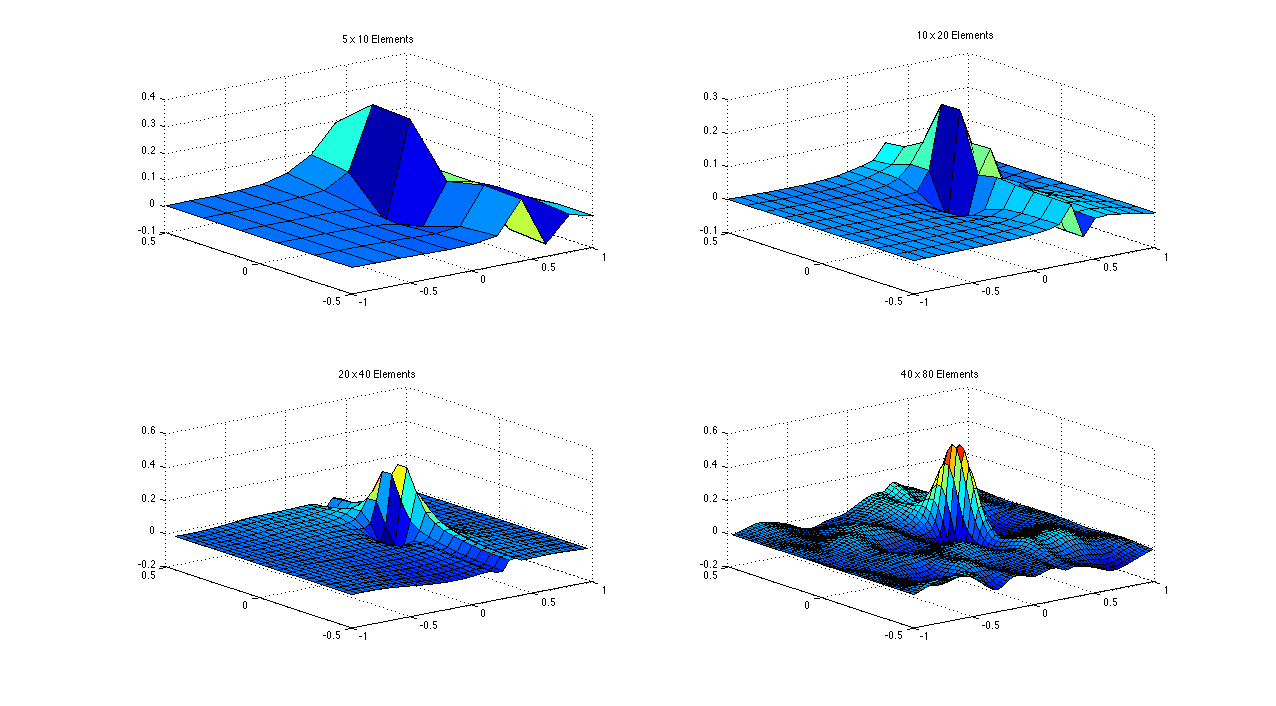
\includegraphics[width=\textwidth]{Figures/waves_in_cavity/waves_in_cavity.png}
\caption{H 3 components obtained after 100 seconds for gaussian function initial condition for various mesh refinements}
\label{WaveConv8}
\end{figure}

\begin{figure}
\includegraphics[width=\textwidth]{Figures/waves_in_cavity/waves_in_cavity_section_delta.png}
\label{WaveConv9}
\end{figure}

\begin{figure}
\includegraphics[width=\textwidth]{Figures/waves_in_cavity/waves_in_cavity_section_gauss.png}
\label{WaveConv10}
\end{figure}


% TODO - non-zero beta values

% TODO - CHECH THAT THIS IS ACTUALLY TRUE

% TODO - 

% TODO - why is this? Are gaussian initial conditions actually better in the long run??

%ConvergeOfWaveShapeWithH:
%-> this was measured after 10 cycles (is that enough for convergence? Who knows?)
%-> NOTE: I NEED TO RUN THIS WITH A HIGHER P AND A BETTER INITIAL CONDITION METHINKS....!! WAAAA!!!

% TODO - EVENTUALLY...! Convergence with P
% \begin{figure}
% \includegraphics[width=\textwidth]{Figures/2DPlate/WaveShapes/ConvergeOfWaveShapeWithP.png}
% \caption{Converge of wave shape with shape function order}
% \label{WaveConv3}
% \end{figure}

% \begin{figure}
% \includegraphics[width=\textwidth]{Figures/matlab/emptyplot.png}
% \caption{Convergence of wave shape measured at a point in space}
% \label{WaveConv4}
% \end{figure}

% \begin{figure}
% \includegraphics[width=\textwidth]{Figures/matlab/emptyplot.png}
% \caption{Error at same point in space as a function of time for various values of p (end every cycle)}
% \label{WaveConv5}
% \end{figure}

% \begin{figure}
% \includegraphics[width=\textwidth]{Figures/matlab/emptyplot.png}
% \caption{Error at same point in space as a function of time for various values of h (end every cycle)}
% \label{WaveConv6}
% \end{figure}

% \subsection{Propagation Constant}
% $\beta$ non-zero runs
% TODO: Change beta and show that the waves change as expected. Try to explain this in terms of the significance of Beta??
% \subsection{conclusion}

\section{FFT Spectrums}

Determination of frequency components of a time domain solution to maxwells equations is commonly done by a fourier transform to frequency space. The following spectrum was obtained by a Discrete Fourier Transform of a signal obtained from a finite element simulation. Peaks corrispond to resonant frequencies - known analytical values for resonant frequency are plotted for comparison.

\begin{figure}
\includegraphics[width=\textwidth]{Figures/matlab/Spectrums/GoodSpectrum.png}
\caption{Spectrum obtained by FFT from a timestep of 0.13E-03, 3,286,002 timesteps and 3200 elements. First order shape functions were used. A blackman window was used to reduce noise.}
\label{Spectrum1}
\end{figure}

% TODO - MAYBE DO WITHOUT A BLACKMAN WINDOW AND WITH A DELTA-FUNCTION INIT COND
% 
% \subsection{Window Functions}
% 
% \begin{figure}
% \includegraphics[width=\textwidth]{Figures/matlab/emptyplot.png}
% \caption{Spectrums with and without a window function}
% \label{WindowFFT1}
% \end{figure}
% 
% Quantify the noise (lowest possible cutoff frequency maybe, or cutoff freq difference)

\subsection{Peak Detection}

\subsubsection{Timestep And Cut-Off Frequencies}

% TODO - higher than Nyquist frequency??

% I need to determine a cut-off frequency?? What strategies do I have?
% 
% plot histogram for various differnt types of spectrum to show differences...! A BAD spectrum should have a BAD histogram
% Plot histogram to a number of ANALYTICAL frequencies with different samplings and spectrum richness (maybe) ??

The highest frequency component which can be indentified from a time-domain signal sampled at frequency $f_{s} = \frac{1}{T}$ where $T$ is the sampling time interval is given by:

$$f_{max} = \frac{f_s}{2} = \frac{1}{2T} $$

This introduces a theoretical upper bound on the spectrum obtained based on sampling frequency. In practice since the sampling interval used is the simulation time step then an upper limit will also be imposed by the stability criterion:

% TODO: STABILITY CRITERION

In practice upper limit for a wave domainated simulation will be the same as the time integration timestep of the simulation which is governed by stability conditions.

However as can be seen in \figref{Timestep1} a finite time-domain signal a sufficiently high sampling frequency will also introduces signal noise below this limit. Here the theoretical highest frequency is shown for each plot however we see degredation in the quality of the spectrum below this cut-off frequency. A sufficiently small timestep should be selected to allow the peaks to be clearly distingushed from spectrum noise. A practical measure of this degredation could be ratio of maximum height of spectral noise to minimum height of signal as shown in \figref{Timestep01}. 

%TODO - show this stuff for HARMINV too (to demonstrate that its relevant).

%TODO:CHECK THIS statement
In practice for these simple examples the time step required for solution stability was sufficient to identify the fundamental frequency of interest. However this could be a consideration if frequencies of interest were higher. %TODO - quantify this...! How much higher before it becomes comparible to stability

%TODO: QUANTIFY how much the timestep effects the ACTUAL frequencies (i.e. by finding the CLOSEST PEAK) - because the input signal is the same every time this probably won't be affected too much by frequency %(dt) for a long run. The real difficulty is in identifying the real and fictitious peaks which arise in the frequency determination. 

\begin{figure}
\includegraphics[width=\textwidth]{Figures/matlab/TimestepConvergence/Spectrums4up.png}
\caption{Spectrum obtained from the same signal using different sampling rates. Signal was generated with a 3200 element mesh and p-2 shape functions and a final time of 500s. The lowest sampling frequency corrisponds to the simulation timestep}
%TODO - how many elements.
%TODO - graph titles
\label{Timestep1}
\end{figure}

%TODO: Talk about cutoff frequencies and identifying resonant frequencies. Noise appears. How does this change with time. If I take a longer time for a noisy signal will this get better?

\begin{figure}
\includegraphics[width=\textwidth]{Figures/matlab/TimeStepConvergence/TimeStepConv.png}
\caption{Error in resonant frequency maximum against sampling period. Same signal used as in \figref{Timestep1}.}
%TODO - how many elements.
%TODO - graph titles
\label{Timestep01}
\end{figure}

%TODO - do this...!
%\begin{figure}
%\includegraphics[width=\textwidth]{Figures/matlab/emptyplot.png}
%\caption{Ratio of minimum resonant frequency component to maximum noise for the first 3 frequencies vs sampling frequency. Same signal used as in \figref{Timestep1}.}
% [or some other measure of how easy it is to extract frequencies - maybe based on histograms?? ]
%\label{Timestep0}
%\end{figure}

% \begin{figure}
% \includegraphics[width=\textwidth]{Figures/matlab/emptyplot.png}
% \caption{Frequencies obtained by sampling a analytical generated spectrum}
% \label{Timestep3}
% \end{figure}

\subsubsection{Peak Resolution}
Signals of finite length undergo a spectral leakage under fourier transform. As a result a shorter sample length results in noise appearing in the a spectrum with wider, badly-resolved peaks as shown in \figref{Period1}. A signal of length $5 \times 10^4$ is sufficient to capture the resonant frequencies with an error of $3 \times 10^6$.

%What is the minimum time I need to accurately capture ths signal at the accuracy required?
% note: more accuracy MEANS that we need much longer runs. No good having a more accurate wave...we also need a more accurate FFT...! So to capture a p3 accuracy with the same level of accuracy we need to run for how many time longer?? :)

% TODO Whats the minimum time (in general) that I need to remove the FFT transform error completely? :)

% TODO: Expression of dependence between timestep and resolution

\begin{figure}
\includegraphics[width=\textwidth]{Figures/matlab/PeriodConvergence/Spectrums4up.png}
\caption{Spectrum obtained from signal using different signal periods. Signal were generated with a timestep of 0.95E-02 using a mesh of 200 elements and p-1 shape functions}
\label{Period1}
\end{figure}

\begin{figure}
\includegraphics[width=\textwidth]{Figures/matlab/PeriodConvergence/PeriodConvergenceManual.png}
\caption{Error in calulations of resonant frequencies obtained against signal length}
\label{Period2}
\end{figure}

%TODO - same for analytical signals made of 1,3,10 \& 100 frequency components
%Use an analytical soltuion to identify (depending on richness of spectrum) the kind of accuracy I can expect to obtain after a FFT.

\subsubsection{Lorentzian Fitting}

In \figref{LorentzFit1} we see a number of resonant peaks fitted with a Lorentzian curve given by:

$$
L(x)=\frac{1}{\pi} \frac{\frac{1}{2}\Gamma}{ (x-x_0)^2 + (\frac{1}{2}\Gamma)^2}
$$

where $x_0$ is the center and $\Gamma$ is a width parameter. The Lorentzian function is commonly used to overcome the peak broadening associated with spectral leakage. In practice however fitting a lorentz curve reliably for narrow peak widths using a least squares method was complicated. However for peaks with less a bad resolution an improvement in the resolution was observed as shown in \figref{LorentzFit2}. This difficulty with fitting is one of the motivations for using the Filter Diagonalisation Method presented later.

\begin{figure}
\includegraphics[width=\textwidth]{Figures/matlab/Lorentz/LorentzFitManual.png}
\caption{Resonant peaks fitted with Lorentz curve at various periods showing the lorentz curve fits as spectrum resolution increases}
\label{LorentzFit1}
\end{figure}

\begin{figure}
\includegraphics[width=\textwidth]{Figures/matlab/Lorentz/LorentzFitPeriodConv.png}
\caption{Results showing the difference obtained by using a Lorentz fit at low periods. Resonably results can be obtained from very short runs in this way. However for longer runs the lorentz fit implementation was less reliable.}
\label{LorentzFit2}
\end{figure}

%\subsection{Spectral Richness}
%Dependece of spectral richness on initial conditions. Dependence of peak height and sharpness on intial conditions too [ maybe this should go somewhere else]

\begin{figure}
\includegraphics[width=\textwidth]{Figures/matlab/harminvr/InitCondHarminv.png}
\caption{Error vs Time for different types of initial conditions produced with FDM method}
\label{InitCond1}
\end{figure}
%delta/gaussian/multiple gaussians(10)/narrow gaussians

%Initial Condition Optimisation:
%\begin{figure}
%\includegraphics[width=\textwidth]{Figures/matlab/emptyplot.png}
%\caption{L2 norm error in the wave shapes against time for different types of initial conditions}
%\label{InitCond2}
%\end{figure}

% \subsubsection{Symmetry}
% \begin{figure}
% \includegraphics[width=\textwidth]{Figures/matlab/emptyplot.png}
% \caption{Spectrum from point with low symmetry and spectrum obtained from same simulation at a point with a high symmetry}
% \label{SymmDep1}
% \end{figure}

% Mesh dependence of initial condition:
% \begin{figure}
% \includegraphics[width=\textwidth]{Figures/matlab/emptyplot.png}
% \caption{Wave vs time for the same gaussian with different mesh sizes}
% \label{SymmDep2}
% \end{figure}

% TODO: Discussion on how finer meshes can capture a better spectrum due to initial condition containing a richer spectrum.

%\subsubsection{Components}
%
%\begin{figure}
%\includegraphics[width=\textwidth]{Figures/matlab/emptyplot.png}
%\caption{Spectrums obtained after 15 cycles}
%\label{CompDep2}
%\end{figure}

% TODO: Different components dominate in different cycles. Can I change the initial conditions to affect this?
%TODO - try to show that spectrums are richer for narrower gaussians??
%TODO(maybe): excite a single component... (?)

%\subsection{Obtaining Data}
%Quality factor...? Should I even mention this?

%\subsection{Conclusion}
%Limitations of FFT. Advantages of FFT (can see the spectrum)

\section{Filter Diagonalization Method}

% V. A. Mandelshtam and H. S. Taylor, "Harmonic inversion of time signals," J. Chem. Phys. 107 (17), 6756-6769 (1997). Erratum, ibid. 109 (10), 4128 (1998).
Limitations with FFT include the number of cycles required for optimal accuracy and the difficulty of lorentz fitting as the peak width gets narrower. The Filter Diagonalization is a popular method that addresses these issues and produces good results in much shorter times. The following are a list of results obtained using the Filter Diagonalization Method. However it is sometimes desirable to also use FFT in order to have a visible spectrum and a more complete picture of spectral content.

Signals were found to sometimes contain additional frequencies or to miss frequencies - but this could be corrected by using a higher number of basis functions.

%when signal consists of arbitrary number...
%TODO - getting rid of additional modes. When do these addtional modes appear? What happens if a run is too long? What happens if its too short.
%--> We get the Q for free (HOOOOW???)

% \begin{figure}
% \includegraphics[width=\textwidth]{Figures/matlab/emptyplot.png}
% \caption{Good spectrum and results obtained from FDM}
% \label{HarmivSpectrum1}
% \end{figure}
% 
% \begin{figure}
% \includegraphics[width=\textwidth]{Figures/matlab/emptyplot.png}
% \caption{Bad spectrum and results obtained from FDM method}
% \label{HarmivSpectrum2}
% \end{figure}
% TODO  FDM and how to optimise. Discuss crap spectrums producing usable results. Discuss fictitious/additional modes and how to get rid of them.......!!

\begin{figure}
\includegraphics[width=\textwidth]{Figures/matlab/harminvr/ConvergenceForDifferentDtHarminv.png}
\caption{Convergence of FDM results for various signal lengths for two different sampling intervals. Note that these sampling intervals also corrispond to time integration timestep. Results are compared with convergence results obtained from the same data for FFT.}
\label{HarmivSpectrum3}
\end{figure}

\begin{figure}
\includegraphics[width=\textwidth]{Figures/matlab/harminvr/HarminvConvergencePlots.png}
\caption{Error in FDM calculations obtained by mesh refinement using 50, 200 and 800 elements for p1 calculations}
\label{HarmivSpectrum4}
\end{figure}

%TODO - Harminv is x times better. Compare them...! Identifying fictitious modes

%\subsection{Initial Condition Dependence}
%show different initial conditions (gaussian, delta, sigma, number of gaussians) - same plot as before with Harminv. Demonstrate difference in initial conditions.

%TODO: is FDM more or less sensitive to initial condition time steps?

%\subsection{Window Functions}

% \begin{figure}
% \includegraphics[width=\textwidth]{Figures/matlab/emptyplot.png}
% \caption{Convergence with window length}
% \label{HarmivWindow1}
% \end{figure}

% \begin{figure}
% \includegraphics[width=\textwidth]{Figures/matlab/emptyplot.png}
% \caption{Convergence with window start time for different p/h}
% \label{HarmivWindow2}
% \end{figure}
